\chapter{Coordinates}
\index{coordinates|hyperbf}

%-----------------------------------------------------------------------------
\section{Local Reference Orbit}
\label{s:ref}
\index{reference orbit|hyperbf}


\begin{figure}[!b]
  \centering
  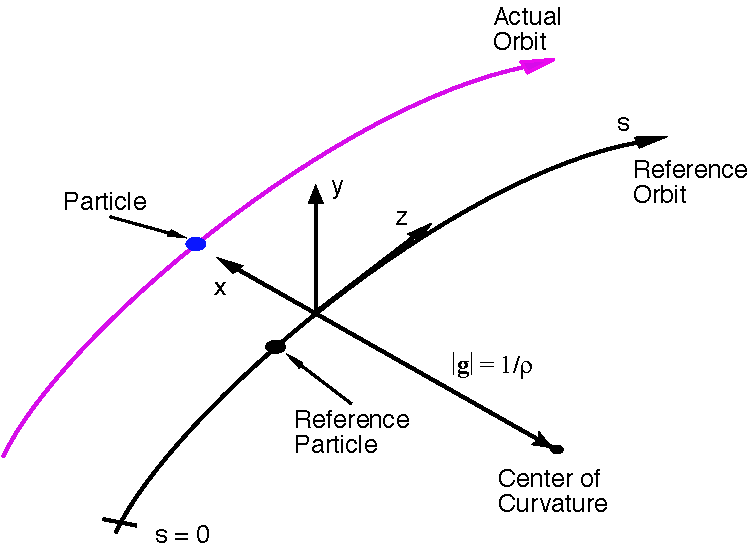
\includegraphics[height=8.4cm]{local-coords.pdf}
  \caption[The Local Reference System.]
{The local reference coordinate system. By construction, a particle's
$z$ coordinate is zero.  This is not to be confused with the phase
space $z$ coordinate (\sref{s:phase.space}).  The curvature vector
$\bfg$ points towards the center of curvature and has a magnitude of
$1/\rho$ where $\rho$ is the bending radius.}
  \label{f:local.coords}
\end{figure}

The \vn{local reference orbit} is the curved path used to define a
coordinate system for particles as shown in
Figure~\ref{f:local.coords}. At a given time $t$, a particle's
position can be described by a point on the reference orbit a distance
$s$ relative to the reference orbit's zero position plus a transverse
offset. This point on the reference orbit is used as the origin of the
local $(x, y, z)$ coordinate system with the $z$--axis tangent to the
reference orbit and pointing in the direction of increasing $s$. The
$x$ and $y$--axes are perpendicular to the reference orbit. If the
lattice has no vertical bends, the $y$--axis is in the vertical
direction and the $x$--axis is in the horizontal plane. Notice that by
construction, the particle is always at $z = 0$. The coordinate system
so constructed is called the \vn{``local coordinate system''} or sometimes
the \vn{``laboratory coordinate system''} when there is need to
distinguish it from the \vn{``element coordinate system''}
(\sref{s:misalign.track}).

\index{sbend}\index{rbend}
\index{crystal}\index{mirror}\index{entrance_end}
\index{exit_end}\index{patch}
In \bmad, a lattice is comprised of a sequence of elements such as
quadrupoles, bends, RF cavities, etc. Each element has an entrance
point, an exit point, and a reference curve between them. For a
\vn{bend} (\sref{s:bend}), the reference curve is a segment of a
circular arc. For \vn{crystal} and \vn{mirror} elements, the reference
curve is a zero length bend (\sref{s:mirror.coords}). All other
elements are ``straight''. That is, the reference curve is a straight
line segment. With multiple elements, the reference orbit is
constructed by arranging the elements so that the reference orbit at
exit point of one element coincides, and is collinear with, the
reference curve at the entrance point of the next element. The
reference orbit is then the sum of the reference curves. Exceptions to
this construction method may be made by using \vn{patch}
(\sref{s:patch}) elements which can arbitrarily orient the entrance
point of an element with respect to the exit point of the previous
element. If not specified otherwise, the $s = 0$ position is the
entrance point of the first element.

\index{x_offset}
\index{y_offset}
\index{x_pitch}
\index{y_pitch}
\index{wiggler}
Notice that, in a \vn{Wiggler}, the reference orbit, which is a
straight line, does {\em not} correspond to the orbit that any actual
particle could travel. Typically the physical element is
centered with respect to the reference curve. However, by specifying offsets, 
pitches or a tilt (See \sref{s:offset}), the physical element may be
arbitrarily shifted with respect to its reference curve.  Shifting a
physical magnet with respect to its reference curve generally means
that the reference curve does {\em not} correspond to the orbit that
any actual particle could travel.

Do not confuse this reference orbit (which defines the local
coordinate system) with the reference orbit about which the transfer
maps are calculated (\sref{s:twiss}). The former is fixed by the
lattice while the latter can be any arbitrary orbit.

%-----------------------------------------------------------------------------
\section{Global Coordinates}
\label{s:global}
\index{global coordinates|hyperbf}

The global coordinate system, also called the `floor'' coordinates,
describes the orientation of the reference
orbit with respect to the laboratory coordinate system.  \bmad,
following the \mad\ convention, uses a Cartesian coordinate system
$(X, Y, Z)$ for the global coordinate system, along with three angles
$\theta, \phi, \psi$ used to define the reference orbit's orientation
as shown in Figure~\ref{f:global.coords}. Conventionally, $Y$ is the
``vertical'' coordinate and $(X, Z)$ are the ``horizontal'' coordinates.  
The three angles are defined as follows:
\begin{description}
\item[$\theta$ Azimuth angle:] Angle in the $(X, Z)$ plane 
between the $Z$--axis and the projection of the $z$--axis onto the
$(X, Z)$ plane. A positive angle of $\theta = \pi/2$ corresponds to the
projected $z$--axis pointing in the positive $X$ direction.
\item[$\phi$ Pitch (elevation) angle:] Angle between the $z$--axis 
and the $(X,Z)$ plane. A positive angle of $\phi = \pi/2$ corresponds to
the $z$--axis pointing in the positive $Y$ direction.
\item[$\psi$ Roll angle:] Angle of the $x$--axis with respect 
to the line formed by the
intersection of the $(X, Z)$ plane with the $(x, y)$ plane. A
positive $\psi$ forms a right--handed screw with the $z$--axis.
\end{description}

\begin{figure}
\centering
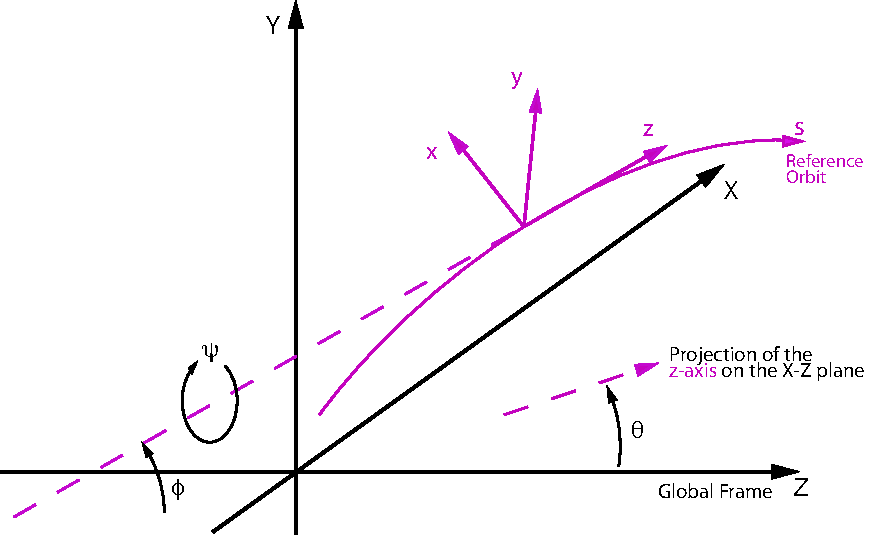
\includegraphics{global-coords.pdf}
\caption{The Global Coordinate System}
\label{f:global.coords}
\end{figure}

\index{beginning statement}
\index{reference orbit!origin in global coordinates}
\index{global coordinates!reference orbit origin}
By default, at $s = 0$, the reference orbit's origin coincides with
the $(X, Y, Z)$ origin and the $x$, $y$, and $z$ axes correspond to
the $X$, $Y$, and $Z$ axes respectively. $\theta$ decreases as one
follows the reference orbit when going through a horizontal bend with
a positive bending angle. This corresponds to $x$ pointing radially
outward. Without any vertical bends, the $Y$ and $y$ axes will
coincide, and $\phi$ and $\psi$ will both be zero. The \vn{beginning}
statement (\sref{s:beginning}) in a lattice file can be use to
override these defaults.

\index{MAD}
Following \mad, the global position of an element is characterized by
a vector $\Bf V$ 
\Begineq
  \Bf V = 
  \begin{pmatrix}
    X \\ Y \\ Z 
  \end{pmatrix}
\Endeq
The orientation of an element is described by a unitary matrix $\Bf
W$.  The column vectors of $\Bf W$ are the unit vectors spanning the
local coordinate axes in the order $(x, y, s)$. $\Bf W$ can be
expressed in terms of the angles $\theta$, $\phi$, and $\psi$ via the
formula
\Begineq
  \Bf W = \Bf W_\Theta \, \Bf W_\Phi \, \Bf W_\Psi
\Endeq
where
\Begineq
  \Bf W_\Theta = 
  \begin{pmatrix}
    \cos\theta  & 0 & \sin\theta \\
    0           & 1 & 0          \\
    -\sin\theta & 0 & \cos\theta 
  \end{pmatrix}, \quad
  \Bf W_\Phi = 
  \begin{pmatrix}
    1 & 0 & 0                \\
    0 & \cos\phi  & \sin\phi \\
    0 & -\sin\phi & \cos\phi 
  \end{pmatrix}, \quad
  \Bf W_\Psi = 
  \begin{pmatrix}
    \cos\psi & -\sin\psi & 0 \\
    \sin\psi &  \cos\psi & 0 \\
    0        &  0        & 1                
  \end{pmatrix}
\Endeq
\index{MAD}
\bmad, again following \mad, computes $\Bf V$ and $\Bf W$ by starting
at the first element of the lattice and iteratively using the
equations
\Begineqs
  \Bf V_i &=& \Bf W_{i-1} \, \Bf L_i + \Bf V_{i-1}, 
    \label{vwlv} \\
  \Bf W_i &=& \Bf W_{i-1} \, \Bf S_i
    \label{wws}
\Endeqs
$\Bf L_i$ is the displacement vector for the $i$\Th element and matrix
$\Bf S_i$ is the rotation of the local reference system of the exit
end with respect to the entrance end. For clarity, the subscript $i$ in 
the equations below will be dripped. For all elements whose
reference orbit through them is a straight line, the corresponding
$\Bf L$ and $\Bf S$ are
\Begineq
  \Bf L = 
  \begin{pmatrix}
      0 \\ 0 \\ L
  \end{pmatrix},
  \quad
  \Bf S = 
  \begin{pmatrix}
      1 & 0 & 0 \\ 
      0 & 1 & 0 \\
      0 & 0 & 1
  \end{pmatrix},
\Endeq

%-----------------------------------------------------------------------

\begin{figure}
  \centering 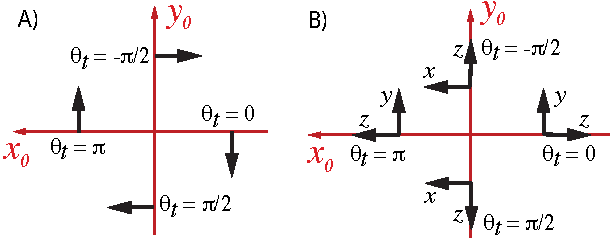
\includegraphics{tilt-bend.pdf} 
\caption[Orientation of the local coordinate system after a bend] {
Orientation of the local coordinate system after a bend shown for a
positive bend angle $\alpha_b$ and for tilt angles $\theta_t$ of 0,
$\pm \pi/2$, and $\pi$. The local coordinates axes before the
bend are labeled $x_0$ and $y_0$ with the $z_0$ axis being directed
into the page.
  }  
  \label{f:tilt.bend}
\end{figure}

%-----------------------------------------------------------------------

\index{rbend}\index{sbend}
\index{rho}\index{tilt}\index{angle}
Where $L$ is the length of the element. For a \vn{bend}, $\Bf L$ and
$\Bf S$ are given by
\Begineq
  \Bf L = \Bf T \, \bftilde L, \quad
  \Bf S = \Bf T \, \bftilde S \, \Bf T^{-1}
  \label{ltl}
\Endeq
where
\Begineq
  \bftilde L = 
  \begin{pmatrix}
    \rho (\cos\alpha_b - 1) \\ 0 \\ \rho \, \sin\alpha_b
  \end{pmatrix}, 
  \quad
  \bftilde S = 
  \begin{pmatrix}
    \cos\alpha_b & 0 & -\sin\alpha_b \\
    0          & 1 & 0           \\
    \sin\alpha_b & 0 & \cos\alpha_b
  \end{pmatrix},
  \quad
  \Bf T = 
  \begin{pmatrix}
    \cos\theta_t & -\sin\theta_t & 0 \\
    \sin\theta_t &  \cos\theta_t & 0 \\
    0            &  0            & 1                
  \end{pmatrix}
  \label{lrca1}
\Endeq
with $\rho$ being the bend radius (\vn{rho}), $\alpha_b$ is the bend
\vn{angle} (\sref{s:bend}), and $\theta_t$ is the \vn{tilt} angle
(\sref{s:offset}). Without a tilt, $\Bf T$ is the unit matrix
resulting in $\Bf L = \bftilde L$ and $\Bf S = \bftilde
S$. Notice that for a bend in the horizontal $X-Z$ plane, a positive
bend \vn{angle} will result in a decreasing azimuth angle $\theta$.

The bend transformation (\Eq{ltl}) is so constructed that the
transformation is equivalent to rotating the local coordinate system
around an axis that is perpendicular to the plane of the bend. This
rotation axis is invariant under the bend transformation. For example,
for $\theta_t = 0$ (or $\pi$) the $y$-axis is the rotation axis and
the $y$-axis of the local coordinates before the bend will be parallel
to the $y$-axis of the local coordinates after the bend as shown in
Fig.~\ref{f:tilt.bend}. That is, a lattice with only bends with
$\theta_t = 0$ or $\pi$ will lie in the horizontal plane (this
assuming that the $y$-axis starts out pointing along the $Y$-axis as
it does by default).  For $\theta_t = \pm\pi/2$, the bend axis is the
$x$-axis. A value of $\theta_t = +\pi/2$ represents a downward
pointing bend.

\begin{figure}
  \centering 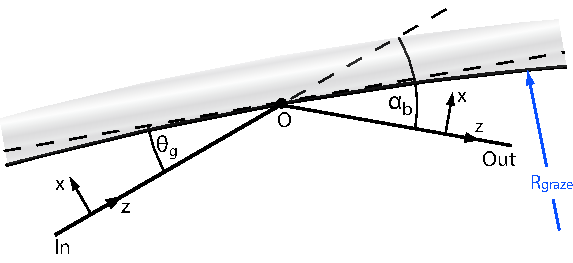
\includegraphics{mirror.pdf} 
\caption[Mirror and crystal geometry] {Mirror and crystal geometry.
The geometry shown here is appropriate for a tilt angle of $\theta_t =
0$.  $\theta_g$ is the graze angle of the incoming (entrance)
reference coordinates, and $\alpha_b$ is the total bend angle of the
coordinates. A) Geometry for a mirror or a Bragg crystal. Point
$\calO$ is the origin of both the local coordinates just before and
just after the reflection/diffraction. B) Geometry for a Laue crystal.
Point $\calO_{out}$ is the origin of the coordinates just after
diffraction is displaced from the origin $\calO_{in}$ just before
diffraction due to the finite thickness of the crystal. here the
``graze'' angles are measured with respect to the line that is in the
plane of the entrance and exit coordinates and perpendicular to the
surface. For Laue diffraction, the user has the option of using the
undiffracted beam (shown in red) as the reference trajectory.
  }  
  \label{f:mirror}
\end{figure}

%-----------------------------------------------------------------------------
\subsection{Crystal and Mirror Element Coordinate Transformation}
\label{s:mirror.coords}

\index{crystal}\index{mirror}\index{tilt}
A \vn{crystal} element (\sref{s:mirror}) diffracts photons and a
\vn{mirror} element (\sref{s:mirror}) reflects them. For a crystal
setup for Bragg diffraction, and for a mirror, the reference orbit is
modeled as a zero length bend with $\bftilde L = (0, 0, 0)$, as shown
in Fig.~\ref{f:mirror}A. Shown in the figure is the geometry
appropriate for a tilt angle of $\theta_t = 0$ (the rotation axis is
here the $y$-axis). Since the mirror or crystal element is modeled to
be of zero length, the origin points (marked $\calO$ in the figure)
of the entrance and exit local coordinates are the same. For Laue
diffraction, the only difference is that $\bftilde L$ is non-zero due
to the finite thickness of the crystal as shown in
Fig.~\ref{f:mirror}B. This results in a separation between the
entrance coordinate origin $\calO_{in}$ and the exit coordinate
origin $\calO_{out}$.

In all cases, the total bending angle is
\begin{align}
  \alpha_b &= \mbox{graze_angle_in} + \mbox{graze_angle_out} &\mbox{! Crystal} \CRNO
  \alpha_b &= 2 \, \mbox{graze_angle}                        &\mbox{! Mirror}
  \label{agg}
\end{align}
With a mirror or Bragg diffraction, the graze angles are measured with
respect to the surface plane. With Laue diffraction the graze angles
are measured with respect to the line in the bend plane perpendicular
to the surface.

For Laue diffraction, the user has the option of using the
undiffracted beam (shown in red) as the reference trajectory.

The orientation of the exit coordinates (the local coordinates after
the reflection) are only affected by the element's tilt and graze
angle parameters and is independent of all other parameters such as
the radius of curvature of the surface, etc. The local $z$-axis of the
entrance coordinates along with the $z$-axis of the exit coordinates
define a plane which is called the element's \vn{bend plane}.  For a
mirror, the graze angle is a parameter supplied by the user. For a
crystal, the graze angles are calculated so that the reference
trajectory is in the middle of the Darwin curve. Calculation of the
graze angles for a crystal is given in Section~\ref{ss:crystal.ref}.

%-----------------------------------------------------------------------------
\subsection{Patch Element}
\label{s:patch.coords}

\index{patch}\index{tilt}
A \vn{patch} element shifts the reference orbit (\sref{s:patch}).
\Eqs{vwlv} and \eq{wws} are used to propagate the $\Bf W$ matrix through a
\vn{patch}. The $\Bf L$ vector for a patch is
\Begineq
  \Bf L = 
  \begin{pmatrix}
    x_{\text{offset}} \,
    y_{\text{offset}} \,
    z_{\text{offset}}
  \end{pmatrix}
\Endeq
The $\Bf S$ matrix corresponding to a
non--zero \vn{tilt} for a \vn{patch} element is
\Begineq
  \Bf S = 
  \begin{pmatrix}
    \cos\theta_t & -\sin\theta_t & 0 \\
    \sin\theta_t &  \cos\theta_t & 0 \\
    0            &  0            & 1                
  \end{pmatrix}
\Endeq
\index{x_pitch}
The $\Bf S$ matrix corresponding to a non-zero \vn{x_pitch} of a
\vn{patch} element is
\Begineq
  \Bf S = 
  \begin{pmatrix}
    \cos\theta_x & 0 & -\sin\theta_x \\
    0            & 1 & 0             \\
    \sin\theta_x & 0 & \cos\theta_x
  \end{pmatrix}
\Endeq
\index{y_pitch}
where $\theta_x$ is the value of \vn{x_pitch}. Finally, the $\Bf S$
matrix corresponding to a non-zero \vn{y_pitch} of a \vn{patch}
element is
\Begineq
  \Bf S = 
  \begin{pmatrix}
    1 & 0             & 0            \\
    0 & \cos\theta_y  & \sin\theta_y \\
    0 & -\sin\theta_y & \cos\theta_y 
  \end{pmatrix}
\Endeq
where $\theta_y$ is the value of \vn{y_pitch}. 

If a \vn{patch}'s \vn{translate_after} is set to True, the offsets are
applied after the pitches and tilts. In this case, \Eq{vwlv} is
replaced by
\Begineq
  \Bf V_i = \Bf W_{i} \, \Bf L_i + \Bf V_{i-1}, 
\Endeq

%-----------------------------------------------------------------------------
\section{Phase Space Coordinate System}
\label{s:phase.space}
\index{phase space coordinates|hyperbf}

\begin{figure}
\centering 
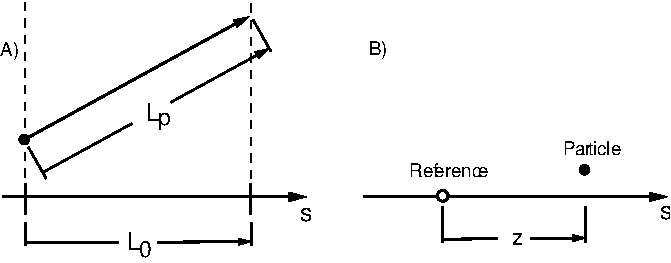
\includegraphics{canonical-z.pdf} 
\caption[Interpreting Canonical $z$ at constant velocity.]
{Interpreting Canonical $z$ at constant velocity: A) The change in $z$
going through an element of length $L_0$ is $L_0 - L_p$.  B) At
constant time, $z$ is the longitudinal distance between the reference
particle and the particle.}
\label{f:canonical.z}
\end{figure}

\bmad uses the canonical phase space coordinates 
\Begineq
  \Bf r(s) = (x, p_x, y, p_y, z, p_z)
\Endeq
The longitudinal position $s$ is the independent variable instead of
the time.  $x$ and $y$, are the reference orbit coordinates given in
\sref{s:ref}.  The canonical momenta $p_x$ and $p_y$ are
normalized by the reference (sometimes called the
design) momentum $P_0$
\begin{align}
  p_x = &\frac{P_x}{P_0} \\
  p_y = &\frac{P_y}{P_0}
\end{align}
where $P_x$ and $P_y$ are respectively the $x$ and $y$ canonical momentums.

\index{lcavity}\index{rfcavity}
The canonical $z$ coordinate is 
\begin{align}
  z(s) &= -\beta(s) \, c \, (t(s) - t_0(s)) \CRNO
    &\equiv - \beta(s) \, c \, \Delta t(s)
  \label{zbctt}
\end{align}
$t(s)$ is the time at which the particle is at position $s$, $t_0(s)$
is the time at which the reference particle is at position $s$, and
$\beta$ is $v/c$ with $v$ being the particle velocity (and not the
reference velocity). The reference particle is, by definition,
``synchronized'' with elements whose fields are oscillating and therefore the
actual fields a particle will see when traveling through such an
element will depend upon the particle's canonical $z$. For example,
the energy change of a particle traveling through an \vn{lcavity} or
\vn{rfcavity} are $z$ dependent as shown in \Eqs{egl2p} and \eq{eev2p}.

If the particle's velocity is constant, and is
the same as the velocity of the reference particle (for example, at
high energy where $\beta = 1$ for all particles), then $\beta \, c \,
t$ is just the path length. In this case, the change in $z$ going
through an element is
\Begineq
  \Delta z = L_0 - L_p
\Endeq
where, as shown in Figure~\ref{f:canonical.z}A, $L_0$ is the path
length of the reference particle (which is just the length of the
element) and $L_p$ is the path length of the particle in traversing
the element.  Another way of interpreting canonical $z$ is that, at
constant $\beta$, and constant time, $z$ is the longitudinal distance
between the particle and the reference particle as shown in
Figure~\ref{f:canonical.z}B. with positive $z$ indicating that the
particle is ahead of the reference particle.

Do not confuse the canonical $z$ with the $z$ that is the particle's
longitudinal coordinate in the local reference frame as shown in
Figure~\ref{f:local.coords}. By construction, this latter $z$ is
always zero.

Notice that if a particle gets an instantaneous longitudinal kick so
that $\beta$ is discontinuous then, from \Eq{zbctt}, canonical $z$ is
discontinuous even though the particle itself does not move in
space. In general, from \Eq{zbctt}, The value of $z$ for a particle at
$s_2$ is related to the value of $z$ for the particle at $s_1$ by
\Begineq
  z_2 = \frac{\beta_2}{\beta_1} \, z_1 - 
  \beta_2 \, c \, (\Delta t_2 - \Delta t_1)
  \label{zbbzb}
\Endeq
$\Delta t_2 - \Delta t_1$ can be interpreted as the difference in
transit time, between the particle and the reference particle, in going
from $s_1$ to $s_2$.

The longitudinal canonical momentum $p_z$ is given by
\begin{equation}
  p_z = \frac{\Delta P}{P_0} \equiv \frac{P - P_0}{P_0}
\end{equation}
where $P$ is the momentum of the particle. For ultra--relativistic particles
$p_z$ can be approximated by
\begin{equation}
  p_z = \frac{\Delta E}{E_0}
\end{equation}
\index{lcavity}
where $E_0$ is the reference energy (energy here always refers to the
total energy) and $\Delta E = E - E_0$ is the deviation of the
particle's energy from the reference energy. For an \vn{Lcavity}
element (\sref{s:lcav}) the reference momentum is {\it not} constant
so the tracking for an \vn{Lcavity} is not canonical.

\index{phase space coordinates!MAD convention}
\index{MAD!phase space convention}
\mad uses a different coordinate system where $(z, p_z)$ is
replaced by $(-c\Delta t, p_t)$ where $p_t \equiv \Delta E / P_0
c$. For highly relativistic particles the two coordinate systems are
identical.

\index{paraxial approximation}
\index{bmad_standard!tracking method}
\vn{Bmad_standard} (\sref{c:methods}) tracking and transfer matrix
calculations use the small angle (paraxial) approximation where it is
assumed that $p_x, p_y \ll 1$. With this approximation, the
relationship, between the canonical momenta and the slopes $x' \equiv
dx/ds$ and $y' \equiv dy/ds$ is
\begin{align}
  x' &\approx \frac{p_x - a_x}{1 + p_z} (1 + g x) \\
  y' &\approx \frac{p_y - a_y}{1 + p_z} (1 + g x) 
  \label{xpa1p}
\end{align}
$\Bf a = q \, A / c \, P_0$ is the normalized vector potential, $g =
1/\rho$ is the curvature function with $\rho$ being the radius of
curvature of the reference orbit and it has been assumed that the
bending is in the $x$--$z$ plane. 

With the paraxial approximation, and in the relativistic limit, the
change in $z$ with position is
\Begineq
  \frac{dz}{ds} = -g \, x - \frac{1}{2} (x'^2 + y'^2)
\Endeq
This shows that in a linac, without any bends, the $z$ of a particle
always decreases.

\index{phase space coordinates!PTC convention}
\index{FPP/PTC!phase space convention}
For those programmers using the PTC\index{PTC/FPP}
software package directly (ignore
this if you don't know what is being talked about here), \'Etienne Forest uses,
by default, a different coordinate system where $(z, p_z)$ is replaced
by $(p_z, -z)$. However, PTC also has the ability to switch to the
$(p_t, c \Delta t)$ coordinate system.

A particle can also have a spin. The spin is characterized by the
spinor $\Psi = \left( \psi_{1}, \psi_{2} \right)^{T}$ where
$\psi_{1,2}$ are complex numbers (\sref{s:spin.dyn}).

%-----------------------------------------------------------------------------
\section{Photon Phase Space Coordinate System}
\label{s:photon.phase.space}
\index{photon!phase space coordinates|hyperbf}

The phase space coordinates $(x, p_x, y, p_y, z, p_z)$ for a photon
are the same as for a particle with $v = c$. The photon frequency $\omega$ and
wave number $k$ are given by the standard formulas
\begin{align}
  \omega &= \hbar \, c \, P_0 (1 + p_z) \CRNO
  k &= \frac{2 \, \pi}{\lambda} = \frac{\omega}{c}
\end{align}

In addition to the above, a photon has
four extra parameters $E_x, \phi_x$, and $E_y, \phi_y$ specifying the
intensity and phase of the field along the $x$ and $y$ axes.
\Begineqs
  E_x (\Bf r, t) &\sim |E_x| \, e^{i (k \, z - \omega \, t + \phi_x)} \CRNO
  E_y (\Bf r, t) &\sim |E_y| \, e^{i (k \, z - \omega \, t + \phi_y)} \CRNO
\Endeqs
The normalization between field and intensity is determined by the
individual simulation programs and is not part of the \bmad standard.

%-----------------------------------------------------------------
\section{RF timing issues}
\label{s:rf.time}

\index{lcavity}\index{rfcavity}
When a particle passes through an \vn{lcavity} or \vn{rfcavity}
element, the kick that it gets is the sum of kicks due to the
fundamental mode, HOM couplers, short-range wakes, and long-range
wakes. For this discussion only the fundamental mode and long-range
wakes need be considered. The fundamental mode and long-range wake
kicks are time dependent but how this time dependence is handled 
differently as explained below.

The kick due to the fundamental mode is based on the particle's $z$
phase space coordinate as shown in \Eq{egl2p} and \Eq{eev2p}. In a
storage ring or recirculating linac a particle goes through the same
cavity multiple times. In such a situation, if the distance from a
cavity back to itself is not a multiple of the fundamental mode
wavelength the simulation will not be self consistent. This can be
seen by a simple example: In a storage ring, a particle simulated by
\bmad traveling on the reference orbit with zero $z$ will never see a
kick from the fundamental mode of a cavity with zero phase
offsets. But, in reality, if the length of the ring is not a multiple
of the fundamental mode wavelength, there will be kicks. The choice to
have \bmad behave unphysically was made since it can be very confusing
otherwise. For example, it is potentially very confusing to see
non-zero closed orbits when one is not expecting it.

On the other hand, the long-range wakes cannot be synchronized to the
$z$ coordinate since, in general, their frequencies are not
commensurate with the fundamental mode frequency. For simulating the
long-range wakes, the kick is thus, by necessity, tied to the absolute
time. The exception is that a wake associated with the fundamental
mode will also use $z$ to determine timing.
